\documentclass{dissertation}
%\documentclass[print]{dissertation}
%\documentclass[print,draft]{dissertation}

\usepackage{pdfpages}
\usepackage{bibentry}

\hyphenation{TestRoots WatchDog proj-ect proj-ects Ec-lipse two-fold clie-nts Mo-cki-to wide-spread}
\newcommand{\sparkline}[1]{$\vcenter{\hbox{\includegraphics[scale=0.04]{#1}}}$}

\makeglossaries

\newcommand*{\origrightarrow}{}
\let\oldarrow\textrightarrow
\renewcommand*{\textrightarrow}{\fontfamily{cmr}\selectfont\origrightarrow}
\loadglsentries[main]{glossary}

\input{abbreviations}

\begin{document}

%% Specify the title and author of the thesis. This information will be used on
%% the title page (in title/title.tex) and in the metadata of the final PDF.
\title{Massivizing {FAIR,} {efficient,} and sustainable workflows for Bioinformatics.}
\author{Michael Robin}{Crusoe}

%% Use Roman numerals for the page numbers of the title pages and table of
%% contents.
\frontmatter

\begin{titlepage}

\begin{center}

%% Extra whitespace at the top.
\vspace*{2\bigskipamount}

%% Print the title.
{\makeatletter
\titlestyle\bfseries\LARGE\@title
\makeatother}

%% Print the optional subtitle.
{\makeatletter
\ifx\@subtitle\undefined\else
    \bigskip
    \titlefont\titleshape\Large\@subtitle
\fi
\makeatother}

\end{center}

\cleardoublepage
\thispagestyle{empty}

\begin{center}

%% The following lines repeat the previous page exactly.

\vspace*{2\bigskipamount}

%% Print the title.
{\makeatletter
\titlestyle\bfseries\LARGE\@title
\makeatother}

%% Print the optional subtitle.
{\makeatletter
\ifx\@subtitle\undefined\else
    \bigskip
    \titlefont\titleshape\Large\@subtitle
\fi
\makeatother}

%% Uncomment the following lines to insert a vertically centered picture into
%% the title page.
%\vfill
%\includegraphics{title}
\vfill

%% Apart from the names and dates, the following text is dictated by the
%% promotieregelement.

{\Large\titlefont\bfseries ACADEMISCH PROEFSCHRIFT}

\bigskip
\bigskip

ter verkrijging van de graad Doctor aan

de Vrije Universiteit Amsterdam,

op gezag van de Rector Magnificus prof.~dr.~V.~Subramaniam,

in het openbaar te verdedigen

ten overstaan van de promotiecommissie

van de Faculteit der Bètawetenschappen

op 1 januari 2024 om 00:00 uur

in [de aula / het auditorium] van de universiteit,

De Boelelaan 1105

\bigskip
\bigskip

door

\bigskip
\bigskip

%% Print the full name of the author.
\makeatletter
{\Large\titlefont\bfseries\@firstname\ \titleshape{\MakeUppercase{\@lastname}}}
\makeatother

\bigskip
\bigskip

%% Extra whitespace at the bottom.
\vspace*{2\bigskipamount}

\end{center}

\clearpage
\thispagestyle{empty}

%% The following line is dictated by the promotieregelement.
%\noindent Dit proefschrift is goedgekeurd door de

%% List the promotors (supervisors).
\medskip\noindent
\begin{tabular}{l}
    promotoren: Prof. dr.\ ir.\ A.\ Iosup\\
    copromotor: Prof. S.\ Ablen
\end{tabular}

\bigskip
\noindent Samenstelling promotiecommissie:

%% List the committee members, starting with the Rector Magnificus and the
%% promotor(s) and ending with the reserve members.
\medskip\noindent
\begin{tabular}{p{4.5cm}l}
    Rector Magnificus, & voorzitter \\
    Prof.\ dr.\ ir. \ A.\ Iosup, & Vrije Universiteit Amsterdam \\
    Dr.\ ir.\ A.\ U{\c t}a, & Leiden Universiteit \\

    \medskip
    \mbox{\emph{Onafhankelijke leden:}} & \\
    Prof.\ dr.\ ir.\ G.J.P.M.\ Houben, & Technische Universiteit Delft \\
    Prof.\ dr. P. Runeson, & Lund Universitet, Sweden \\
    Dr.\ Th.\ Zimmermann, & Microsoft Research, \\ &United States of America \\
    Prof. dr. D. Spinellis, & Athens University of Economics and Business, \\&
    Greece \\
    
    Prof.\ dr.\ ir.\ E.\ Visser, & Technische Universiteit Delft, reservelid \\ \\

    \multicolumn{2}{l}{Prof. dr. D. Spinellis has contributed to the end
    phase of writing \ldots} \\
\end{tabular}

%% Include the following disclaimer for committee members who have contributed
%% to this dissertation. Its formulation is again dictated by the
%% promotieregelement.
%\medskip
%\noindent  %Prof.\ Dr.\ D.\ Spinellis has contributed to the creation of this thesis.

\medskip
\medskip
% TODO Include http://www.win.tue.nl/ipa/?page_id=309
%%\noindent The work in the thesis has been carried out under the auspices of the research school ASCI
(Advanced School for Computing and Imaging).

\medskip
%% Here you can include the logos of any institute that contributed financially
%% to this dissertation.
\vfill
\begin{center}
    \includegraphics[height=0.5in]{title/logos/vu}
    \hspace{2em}
    %\includegraphics[height=0.5in]{title/logos/casimir} \\
    %\includegraphics[height=0.5in]{title/logos/nwo}
    %\\ \vspace{0.5cm}
    %\includegraphics[height=0.5in]{title/logos/asci}
\end{center}
\vfill

\noindent
\begin{tabular}{@{}p{0.2\textwidth}@{}p{0.8\textwidth}}
  \textit{Keywords:} &  \\[\medskipamount]
      \textit{Printed by:} &  \\[\medskipamount]
      \textit{Cover:} &  \\[\medskipamount]
      \textit{Style:} & Atlarge House Style, based on the TU Delft House Style with modifications by Moritz Beller and Laurens Versluis \\& \url{https://github.com/atlarge-research/atlarge-phd-thesis-template} \\[\medskipamount]
\end{tabular}

\medskip
\medskip
\noindent The author set this thesis in \LaTeX\xspace using the Libertinus and Inconsolata fonts.

\vspace{\bigskipamount}

% Copyrighting this is stupid, questionable, and probably illegal, because large parts of the
% thesis have already been published with the copyright resigning with the publisher.
%\noindent Copyright \textcopyright\ 2015 by A.~Einstein

%% Uncomment the following lines if this dissertation is part of the Casimir PhD
%% Series, or a similar research school.
%\medskip
%\noindent Casimir PhD Series, Delft-Leiden 2015-01

%\medskip
\noindent ISBN \ldots

\medskip
\noindent An electronic version of this dissertation is available at \\
\url{https://www.ub.vu.nl/en/}.

\end{titlepage}



%% The (optional) dedication can be used to thank someone or display a
%% significant quotation.
%\dedication{\epigraph{There's no free lunch.
%  }{Alexandru Iosup}}

\tableofcontents

\chapter*{Summary}
\addcontentsline{toc}{chapter}{Summary}
\setheader{Summary}

Your summary.

%\chapter*{Samenvatting}
%\addcontentsline{toc}{chapter}{Samenvatting}
%\setheader{Samenvatting}
%
%{\selectlanguage{dutch}
%
%  Samenvatting in het Nederlands.
%}




\include{acks/acks}

%% Use Arabic numerals for the page numbers of the chapters.
\mainmatter

%% Turn on thumb indices.
\thumbtrue

\nobibliography*

\chapter{Introduction}
\label{introduction}

\begin{abstract}
Sample Abstract.
\end{abstract}


\newpage

\dropcap{T}his is a introductory page.


%Introduction: 2-4 pages; look at existing group work; time-box write for 2 days; send for review & repeat.
%Context
%Problem statement
%Research questions — explicitly, also why they are scientific research questions
%Approach, including focus on methodology
%Contribution, explicitly and with details pointing to the chapters/sections where it appears in the thesis
%Conceptual
%Technical
%Community
%Dissemination
%Thesis reading guide
%Non-plagiarism statement – “I did this stuff, not ChatGPT or someone else”
%Open Science / Reproducibility statement


\section{Background \& Context}
In this thesis, you can reference pictures~\Cref{fig:devmodel} using Cleverref and circles \circled{5}.

\begin{figure}[htb]
	\centering
	\includegraphics[width=0.65\columnwidth]{development_model_without_papers}
	\caption{The stages of the FDD model and their relationship to other
          Software Engineering concepts.}
	\label{fig:devmodel}
\end{figure}

We also have lists:

\begin{enumerate}
  \item Static Analysis~\circled{3} examines program artifacts or
    their source code without executing them~%\cite{wichmann1995industrial}
		, while
 \item Dynamic Analysis~\circled{4} relies on information gathered from their
   execution~%\cite{cornelissen2009systematic}.
\end{enumerate}

Or boxes:

\begin{framed}
This thesis is concerned with the empirical assessment of the state of the art of how developers
drive software development with the help of feedback loops.
\end{framed}

Or code:
\begin{lstlisting}[caption={\textsc{TrinityCore}},label={lst:e1}]
 x += other.x;
 y += other.y;
 z += other.y;
\end{lstlisting}


I hope this helps you get started!
Moritz \& Laurens


\chapter{Methods Included: Standardizing computational reuse and portability with the Common Workflow Language.}
\label{methods-included}

\bibentry{crusoe-methods-2022}

Licensed under "CC BY 4.0, Attribution 4.0 International" \url{http://creativecommons.org/licenses/by/4.0/}

Reproduced here without changes including supplemental material "p54-crusoe-supp.pdf".

%% TODO: investigate using https://ctan.org/pkg/pax to restore the annotations and other embedded links in the included PDFs
\includepdf[pages=-,addtotoc={1,section,1,Introduction,methods-included-introduction,4,section,1,Background on Workflows and Standards for Workflows,methods-included-background,4,subsection,2,Why Workflows?,methods-included-why-workflows,4,subsection,2,{Sidebar:} Monolingual and Polylingual Workflow Systems,cwl-methods-mono-poly,5,subsection,2,Why Workflow Standards?,methods-included-why-standards,6,section,1,Features of the Common Workflow Language Standards,methods-included-features,7,subsection,2,{Sidebar:} The CWL Project and Free/Open Source Software (F/OSS),methods-included-foss,7,subsection,2,Execution of workflows in CWL format,methods-included-wflow-exection,8,subsection,2,When is CWL not useful?,methods-included-not-useful,8,section,1,Open {Source,} Open {Standards,} Open Community,methods-included-open-star,8,subsection,2,The CWL Principles,methods-included-cwl-principles,9,section,1,Conclusion,methods-included-conclusion}]{methods-included.pdf}
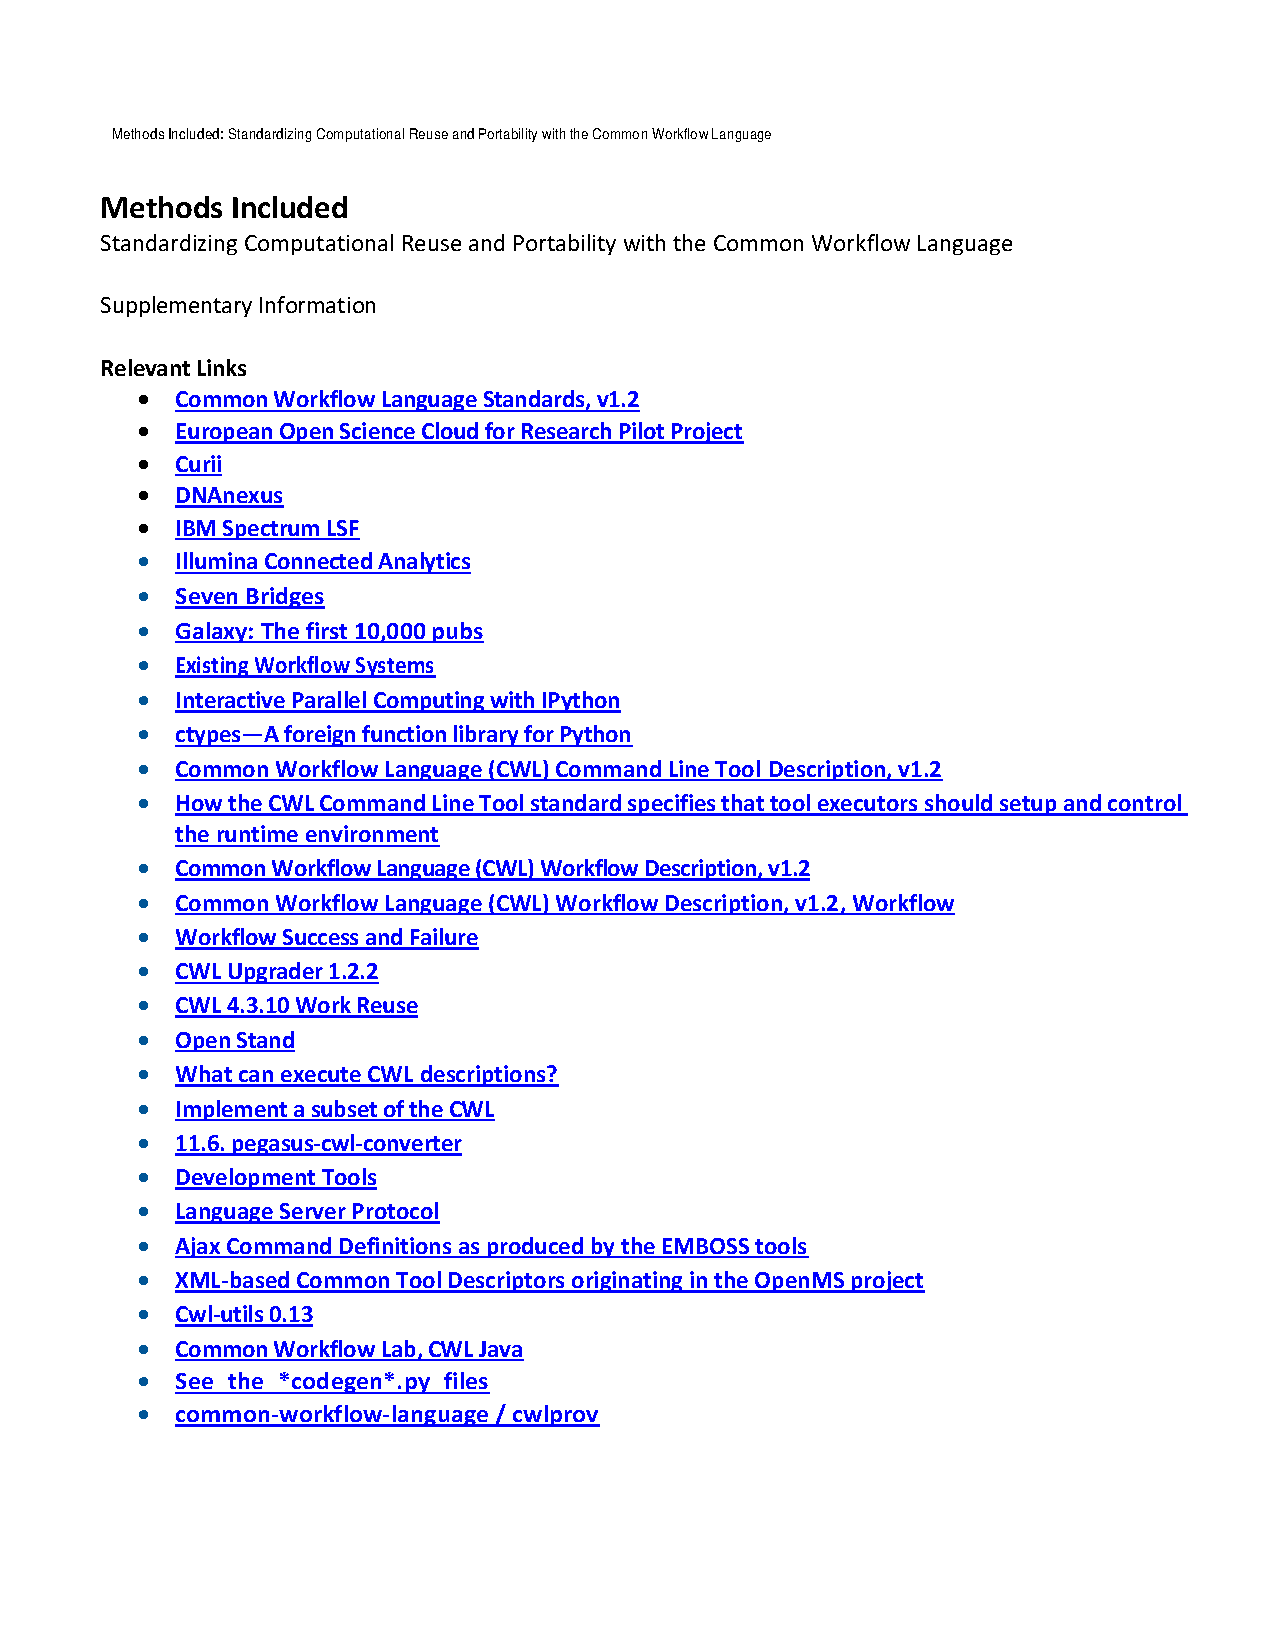
\includepdf[pages=-]{p54-crusoe-supp.pdf}

\chapter{CWL Deep Dive}
\label{cwl-deep-dive}


\dropcap{C}ommon Workflow Language is ...

In \cite{crusoe-methods-2022} we described how the CWL community came to be, the community's goals and ways of working.

In this chapter I will take a deeper dive into the technical decisions made by the CWL Community (of which I'm a co-founder, later CWL Community Engineer and since 2018 the CWL Project Leader).

%Target: IEEE Transactions on Parallel and Distributed Systems (TPDS)
%Audience: future students to explain my work and way of working
%FOCUS ON: 
%Design choices
%Implementation choices
%Practical use
%Lessons learned
%Comparison with state-of-the-art


%Sufficiency / necessity argument: high level comparison with alternatives/competitors
%Repeat qualitative analysis for other popular workflow languages (WDL, SnakeMake, Nextflow, Galaxy)
%sufficient --> has all features
%necessary --> first/only one to have _all_
%Column A1: core workflow patterns (almost all have it) ← evidence + expert interpretation
%A2: conformance test (few have it) ← evidence based
%A3: ... (community developed) ← argumentative
%A4: multiple independent implementations ← evidence based


% Need to explain each decision; for each: what were the alternatives and why weren’t they chosen?
% 
% Relationship with control-flow workflows (systems): (data-flow workflows go inside control-flow workflows, not the other way around)
% 
% Design choices
% 
% Build upon existing standards (POSIX, OCI, YAML, JSON-LD, RDF)
% Separation of concerns: <details needed>
% (often with accompanying Docker format software containers)
% Focus on the workflow author (IDE integrations, syntax choices, future plans)

\section{The Problem of Standardization}

A standard is the named communication of an existing agreement between a group to a larger context. Therefore prior to standardization that group has to come to an agreement and precisely define their shared understanding. Initially the group that became the CWL community looked at codifying an existing workflow and tool description language (specifically Galaxy) as the basis for a standardized workflow language. After a deeper examination it was found by Galaxy core developers that due to Galaxy’s many years of organic growth and an early choice about how to enable templating and advanced command line construction\footnote{Galaxy’s tool description format allows for Python expressions. However the Galaxy workflow engine is written in Python and due to other technical reasons this meant that tool description authors had access to all Galaxy internals from their tool descriptions. Therefore, for other systems to implement the Galaxy tool description format they would need the entire Galaxy Python codebase (or an implementation of it) available as well.} made it unsuitable to codify the Galaxy tool description language directly into a standard. Therefore the decision was made to make a new workflow and tool description language, building on the lessons learned from the multitude of workflow languages and systems before.

Making a new workflow language, even working from the perspective of many decades of collective experience, is not a small undertaking. Add to that the creation of a precise specification, conformance tests, and many implementations and one sees why standardization and the necessary work that both precedes that succeeds standardization needs to be weighed against the potential and likely benefits.

\section{An Idealized Workflow Language}
%<AI->MC: Explain what kinds of issues such a language would address, preferably with brief examples. Then, you can derive naturally the goals. // could go in the Introduction (goals for the next decade, but here we take one step toward standardization)>

Workflow issues circa 2014: 
1. tool/workflow descriptions that depend on engine/platform implementation details are non-portable
2. lack of standard or shared language meant that tool authors or 3rd parties describing tools have to support each workflow system separately. For complex command-line tools, or ones that changed quickly, this maintenance burden was substantial
3. some workflow approaches did not scale well with larger sets of data or increasing complexity of the workflow (common with Make-like systems that encode step names, replica and sample IDs and other organizational details in the filenames assigned to data)
4. Most "in house" workflow systems bake in local computing facility details (names of servers, specific filesystem mount paths) that prevent anyone using even the same code at another institute without (perhaps significant) modification.
5. Existing standards in the workflow space were not relevant to most scientific workflows; instead focused on control-flow and business process workflows.

\subsection{Goals}
Standardized functional portable description of command-line tools and dataflow workflows made up of them
(these descriptions are able to be complete enough to execute)
There should not be implementation or vendor specific details in the specification.
Improve communication and understanding between workflow author and users labels / human friendly identifiers / subworkflows
That data and inputs are explicit and they have identifiers
All the hallmarks of a good workflow system (ASAP) are supported directly or indirectly
Being a good player in the ecosystem by supporting the 17 FAIR Principles where possible. (See section 5 for more details).

\subsection{Non-Goals}
Supporting every theorized workflow construct ; the “Common” in CWL is about targeting the features that are both commonly used by workflow authors and commonly implemented by workflow engines.
(web) service orchestration / interaction with external stateful systems 
Why not? they have state, can go away, not idempotent, not reproducible. (The Taverna experience) Services are not bad, but they need to give the users the workflow and references to the reference data used
Neither business process management nor other control-flow approaches
(no stopping for external decision making, which is not reproducible). CWL tools/workflows could be called from a business process management.
not a strict guarantee of reproducibility

\section{The Design of CWL}
\subsection{Overview}
Two sets of features for the 2 standards
% one visual
\subsection{Design Choices}
\subsubsection{Unit of compute: POSIX command line tools.}

* Supports Goal \#1

* In bioinformatics, command line tools vastly outnumber services and GUIs
* The POSIX application interface is well understood and widely used
* The model in summary: inputs are a list of strings, outputs are written to the filesystem, STDOUT, and STDERR. Assume that exit code of not 0 is an error, this is customizable. CWL v1.2 allows capturing the exit code for further use.
* Services were not chosen as they are too fragile and immature compared to POSIX; experience with Taverna and other systems showed that many advanced concepts are needed to cope. Services are rarely 1st class components of workflow systems, so not a good candidate for a “common” language.

\subsubsection{connection between compute and data into a full workflow (the dataflow model)}
Necessary to have enough information to support Goal \#1 and \#4
We must document all connections between tasks, even those that a user might not be aware of
This enables portability regardless of the execution environment being  distributed or having a shared filesystem. It also enable better provenance tracking
CWL’s object model does not use strings to track file or directory inputs and outputs, instead using a simple dictionary of properties (“class: File” and “class: Directory”). These objects do not assign a path to a File or Directory until just prior to tool execution. Instead Files and Directory have a “location” identifier, and the name of the File or Directory is also stored separately, allowing the location IRI to be meaningful to the workflow engine.
Alternatives:

\subsubsection{file streaming is supported but not required}
A common optimization pattern in hand written workflows
If marked as such, CWL allows File inputs/outputs to be implemented using a named pipe, a.k.a “|”
This allows workflow systems to speed up execution by streaming data into/out-of object stores or directly between tasks
All “type: stdin”, “type: stdout”, and “type: stderr” Inputs/Output have this potential without further specification by the user. Otherwise they can add `streamable: true’ to any Input/Output of `type: File` or `type: File[]`
This was a simple thing to add to the CWL specification, so not adding it was not seriously considered. However, exploitation of this feature has only been done by one engine: toil-cwl-runner.

\subsubsection{no tool to tool IP based communication}
Would violate anti-goal \#1
Ensuring a network path may be non-trivial or not allowed in some workflow execution systems ; implies co-scheduling, which is not very common
Lots of costs to implement this and often not needed, so we kept it out of CWL very early on
CWL has no construct to specify parallel co-scheduling nor port coordination
There are many frameworks and libraries for service orchestration, users are encouraged to use them if that is their need

\subsubsection{syntax choices (balance between readability and using off the shelf libraries for parsing)}
While CWL is regular enough for automated conversion to/from, or programmatic assembly, we knew that users would still be writing/editing by hand (especially during the early phases of adoption) (Goal \#3)
When a design decision came down to an option being more convenient for users versus implementers, we often chose the users. Planned revisions to the standards will include even more user focused design patterns.
Many users of CWL will be causal and infrequently interacting with CWL. By favoring users we make the language more attractive and increase the likelihood of adoption
Examples: map<> syntax simplification; YAML;
JSON? Can’t have comments ; new DSL? Harder to implement, not necessarily more readable for users. XML? gross.

\subsubsection{Review of workflow constructs supported}
(explain why and cross-reference the workflow patterns repository) See \url{https://github.com/common-workflow-library/cwl-patterns/tree/master/workflow_patterns_initiative}

\subsubsection{Optional parts}

To support a diverse ecosystem (Goal \#3). Some workflow engines may not want to / be able to implement all of the CWL syntax
What:
V1.0+: InlineJavascriptRequirement, SchemaDefRequirement, LoadListingRequirement, DockerRequirement, SoftwareRequirement, InitialWorkDirRequirement, EnvVarRequirement, ShellCommandRequirement, ResourceRequirement
V1.1+: WorkReuse, NetworkAccess, InplaceUpdateRequirement, ToolTimeLimit
V1.2+: (abstract) Operation processes (non-runnable, useful for provenance reporting from non-CWL systems), conditional execution of steps using `WorkflowStep.when`

One can use/implement the CWL CommandLineTool standard separate from the entire Workflow standard, if desired
This allows engines and other CWL consumers/produces to make progressively more useful tools while being able to communicate clearly what they support to users (and to fail quickly if given a document they can’t fully execute)
All of these features must be listed by the author of a CWL document, if used, except for conditional workflow steps in CWL v1.2+. Features mentioned under the “hints” section are allowed to be ignored by consumers of the document if they don’t (yet) support them. Features mentioned under “requirements” must be supported, and if they are not available then consumers of the document should fail early and inform the user why.
Feature detection by syntax (instead of these explicit feature flags) was considered and may be implemented in CWL 2.0 to simplify the syntax for the description author.

\subsubsection{Linked data and external ontologies}

Don’t reinvent the wheel, Supports Goals 2,3, 4
File formats are complicated and often very domain specific. Likewise metadata models for workflows and tools
The external ontologies are governed and maintained by experts and contributors, each on their own cadence separate from the CWL standards cadence. Therefore they can be improved/extended without waiting for a new release of CWL
The EDAM ontology is a popular source of identifiers for bioinformatic file formats and it models the relationship between them along with many other useful aspects. For CommandLineTool and Workflow metadata, it is recommended (but not mandatory) to use the schema.org ontology.
Bundling specific baseline versions of some of these ontologies in CWL as a shortcut for users has been considered and might appear in a future version of the standards.
\url{https://www.commonwl.org/v1.1/Workflow.html#Extensions_and_metadata}

\subsubsection{software containers}
Optional, but recommended! Docker format, engine agnostic (Singularity, podman, apptainer, docker, etc..)
Software installation is said to be the hardest problem in bioinformatics and many other research fields
Therefore CWL supports the specification of an recommended (or required) Docker format software container as part of the CommandLineTool specification
This helps (but does not guarantee) reproducibility
Under “DockerRequirement”, tool description authors can specify one of the following: the name of a docker/OCI format image from a registry (defaulting to hub.docker.com but others are allowed) ; a URL to a docker/OCI format image ; an in-place “Dockerfile” format recipe for Docker/OCI format image construction
When CWL began, the Open Container Initiative was in its infancy. It is planned that future versions of the CWL standards will refer to the OCI standards more directly. The Docker engine is not a requirement for fulfilling the “DockerRequirement”, any engine that support the Docker image format (directly or indirectly) is a valid choice by a CWL compliant engine; this includes Singularity, udocker,
\subsubsection{Mechanism for extensions}
Allows and encourages vendors/users to develop/use well marked extensions to the CWL standards
As CWL aims to support features that are “common”ly used by people and “common”ly implemented by engines, it shouldn’t get in the way of those who want to build upon it
Now that CWL is more stable and more widely deployed, getting vendors to experiment with new features and then learning from their experiences provides a better model for stable enhancement
All extensions must be a URL (often abbreviated using the \$namespace feature) and preferably resolve to a web page with more information about the extension. Several features that exist in post v1.0 version of CWL came from vendor extensions: TimeLimit, WorkReuse (previously \url{http://arvados.org/cwl#ReuseRequirement} ), NetworkAccess, InplaceUpdateReqirement, LoadListingRequirement. Like the optional features of CWL, they can be specified under the “hints” section if they can be safely ignored, or under “requirements” if they are necessary for proper execution.
The alternative would be secret extensions/changes that would be hard to detect prior to tool/workflow execution which would hamper reproducibility/ reusability.
\subsubsection{conformance tests}
Need to be able verify the behavior of the various CWL implementations (Goal \#2)
Conformance tests that target different features, their aspects, and combinations of the above along with specified correct output (or a flag that the provided input should result in an error). The tests are tagged with the names of optional features used, if any.
This provides assurances to users that their CWL documents will work in multiple environments, and helps engine authors make progress as they implement CWL features
Conformance tests are developed in conjunction with releases of the CWL standards. They are available under the Apache 2.0 license.
We wrote our own testing framework, but this is a prototype of a plugin to py.test that could be completed.
\subsubsection{Optional support for Javascript in very well defined circumstances}
As the CWL standards don’t aim to cover all possible needs especially when it comes to most extremely badly designed command line interfaces, a script language was chosen as an optional feature.
Users may provide values for certain fields in CWL using ECMAScript 5.1 (commonly known as Javascript). What objects are available to them in that context is tightly defined; no cross talk is allowed; and the order of parsing is explicit
This allows users to work around missing features without having to change the underlying program (which might not be possible or realistic). It also allows for cheap rearrangement of complex object trees without requiring scheduling a task and marshalling/unmarshalling data.
Users must specify that they need the `InlineJavascriptRequirement` under features. To distinguish the javascript from literal strings, it is wrapped in `${ }` for  ECMAScript function body style, or `$( )` for ECMAScript Expression style.
This has been a controversial feature. Many users (and the authors of the CWL standards themselves) would prefer to use Python, but the lack of secure Python VMs prevented this. Currently we are debating on how best to allow users to write CWL Expressions using newer versions of the ECMAScript standard while keeping backward compatibility. ECMAScript 5.1 is from 2011, but newer versions of ECMAScript are not completely backwards compatible with code that targets ECMAScript 5.1.
\subsubsection{Separation of concerns}
There are many audiences for a workflow or tool description and they can be divided into those who execute said description and those who write them.
In designing and refining the CWL standards, maintaining this separation of concerns cleanly was an important sub-goal.
This allows workflow/tool description authors to focus on their analysis and/or communication goals. Likewise it allows workflow engines to focus on optimizing the execution of these same descriptions.
The declarative syntax of CWL, the defined boundaries and expectations, and CWL being a standard and not a library or framework that must be included all give freedom to workflow engines authors to optimize as best they can. It even encourages “vertical engineering” where a workflow system is written, or heavily customized, for a specific technology stack as opposed to the traditional middleware “compatible with everything” approach that sacrifices speed and maintainability for flexibility.
From an engineering perspective, this separation of concerns is at the heart of CWL. Alternatives to this approach were not considered from the moment the founders decided to make a community standard.
\subsubsection{variety of execution models}
single-machine, cluster with a shared filesystem, and distributed
Researchers typically have access to a wide variety of computing capability, and their workflows should not need to be rewritten to be runnable elsewhere. (Portability from Goal \#1)
CWL’s object and execution model allow for execution on a single-machine, compute cluster with a shared filesystem, or distributed execution without a shared filesystem. None of this requires any changes to the tool nor workflow descriptions
Assumptions about paths, directory layouts, and other local details are quite common in hand written workflows. Once these workflow get very large (as they tend to do over time) this can be incredibly time consuming to abstract out. By building this into the CWL standards, everyone benefits without additional work.
As mentioned before, CWL does not represent the a file as a string, but instead as an object with properties, thus forcing the tool description author to be explicit about which inputs are files and which are not. Likewise, when forming a workflow by connecting the inputs and outputs of tools together, one does not do so by using file names or paths (like in a Makefile) but by using identifiers for particular outputs of particular steps which are often meaningful and concise.
5. alternatives not chosen, and why they weren't selected
\subsubsection{Differentiating between data paths and regular strings}
In the CWL object model, which can be queried and manipulated by CWL Parameter References and CWL Expressions, we distinguish between paths (to a file or a directory) and other strings.
While at the time of CommandLineTool execution a filesystem path will be synthesized, at all other times these objects are distinguished by a URI.
This URI might be meaningful to the engine directly (like an object store path) or it might be further transformed or queried internally.

\subsection{Syntax Examples of CWL}

\subsection{Support levels for optional features in CWL runners circa 2024}
% TODO: turn into a table
`toil-cwl-runner`: all of CWL v1.0-v1.2; `InplaceUpdateRequirement` is only supported when using a shared filesystem with the ``--bypass-file-store`` option.


\section{The CWL standards support the 17 FAIR Principles}
It is one of the goals of the CWL project to assist workflow engines/platforms and users in realizing the FAIR principles[3] while not imposing a burden for lack of perfection or completion. When considering the FAIR and CWL we examine not just the context of the workflow and tool descriptions, but also the context of creating, sharing, and executing these descriptions; and finally the context not narrowing the adherence of inbound data to the FAIR principles and increasing the adherence of the FAIR principles for the outbound data.

Rather than attempting to conduct a quantitative study, we focus here on qualitative analysis as the FAIR Principles are just that, principles, and not specific metrics. For specific data types there are specific community led FAIR metrics, but there are no universal FAIR metrics (nor should there be, as “FAIR is not a standard”[4]).
\subsection{To be Findable}
\subsubsection{F1. “(meta)data are assigned a globally unique and persistent identifier”}
In CWL, all items of type File, Directory, Workflow, and CommandLineTool have an identifier which can be “globally unique and eternally persistent” if available, or just locally meaningful. For example, the CWL reference implementation’s use of CWLProv generates random UUIDs for inputs, outputs, and intermediate values, but a workflow platform or service would use registered identifiers.
\subsubsection{F2. “data are described with rich metadata (defined by R1 below)”}
The CWL standards prescribe how Workflow and CommandLineTool descriptions can have arbitrary embedded metadata in a structured way. For generic metadata it is recommend to use the schema.org vocabulary. While community or domain specific metadata is also allowed and encouraged, the CWL standards do not prescribe any particular metadata standard, as that is a decision for specific groups to develop and evolve.
\subsubsection{F3. “metadata clearly and explicitly include the identifier of the data it describes”}
This is automatic for CWL documents, as the metadata is embedded in the data it describes.
\subsubsection{F4. “(meta)data are registered or indexed in a searchable resource”}
There are several registries of workflows, and one in particular (Workflow Hub) has chosen the CWL object model for their workflow metadata model, even for workflows not written using the CWL standards.
\subsection{To be Accessible}
\subsubsection{A1. “(meta)data are retrievable by their identifier using a standardized communications protocol”}
There is no official API for retrieving a CWL document via an identifier. Popular choices include HTTP and the “GA4GH Tool Registry API” (also known as GA4GH TRS). By retrieving a CWL description (data) one then has access to the embedded metadata (if any).

For retrieval of input data for the execution of a CWL workflow or tool, CWL allows for any URI scheme. HTTP(S) is available in all known CWL implementations (modulo local network policies) and many implementations support the relevant object storage protocols. GA4GH has an API specification (GA4GH DRS) for services that convert a data identifier into a platform (and perhaps region) specific URI. Using any of these protocols, their future versions, or entirely new protocols, requires no changes to the CWL standards as long as URI/IRIs are available.
\subsubsection{A1.1 “the protocol is open, free, and universally implementable”}
HTTP, GA4GH TRS, and GA4GH DRS all meet this requirement.
\subsubsection{A1.2 “the protocol allows for an authentication and authorization procedure, where necessary”}
HTTP meets this requirement. For GA4GH TRS they state that “GA4GH recommends the use of the OAuth 2.0 framework (RFC 6749) for authentication and authorization. It is also recommended that implementations of this standard implement and follow the GA4GH Authentication and Authorization Infrastructure (AAI) standard.
While the TRS standard itself does not define any behaviour specific to authorization, given that it hosts and shares publicly available workflows. For future expansion, we recommend that if authorization is needed, that it follows the OAuth 2.0 recommendations as defined above.”
For GA4GH DRS “The DRS implementation is responsible for defining and enforcing an authorization policy that determines which users are allowed to make which requests. GA4GH recommends that DRS implementations use an OAuth 2.0 bearer token, although they can choose other mechanisms if appropriate.”
\subsubsection{A2. “metadata are accessible, even when the data are no longer available”}
Not a guarantee for GA4GH TRS, DRS, or plain HTTP. Possibly guaranteed for workflows registered with the Workflow Hub.
\subsection{To be Interoperable}
\subsubsection{I1. (meta)data use a formal, accessible, shared, and broadly applicable language for knowledge representation.}
Tool and workflow descriptions that conform to the CWL standards are transformable (inclusive of any embedded metadata) to JSON-LD as a pleasant (and purposeful) side effect of the CWL standards being defined in Salad schema language. The reference implementation of CWL has such a capability.

“There are three parts to [the CWLProv] profile:

	CWLProv BagIt, how the resources of an execution are packaged using BagIt
	CWLProv Research Object, how the resources of an execution are related in an RO
	CWLProv PROV, how the workflow execution provenance is modelled in W3C PROV“
\subsubsection{I2. (meta)data use vocabularies that follow FAIR principles}
The vocabularies used in CWL are RDF schema, Salad (which uses Dublin Core terms, RDF, XML, and XSD). Examining these vocabularies in the context of the FAIR principles is out of scope for this paper. The vocabularies used in CWLProv are CWL, ResearchObject, BagIt, and the PROV-Data Model (PROV-DM). User provided vocabularies, such as identifiers for data format types (like the EDAM Ontology), or CWL document metadata (like schema.org), may or may not meet the FAIR principles.
\subsubsection{I3. (meta)data include qualified references to other (meta)data}
All references in the CWL and CWLProv object models are qualified.
\subsection{To be Reusable}
\subsubsection{R1. meta(data) are richly described with a plurality of accurate and relevant attributes}
The CWL standards explicitly support user provided metadata and specifically using the schema.org ontology. There are a number of other specific attributes available in CWL documents as well: ‘label’, ‘doc’, ‘SoftwareRequirement’.
\subsubsection{R1.1. (meta)data are released with a clear and accessible data usage license}
The CWL standards and schemas are released under the Apache 2.0 open source license; likewise the CWLProv profile. Individual CWL documents can embed a license reference using a schema.org annotation which is picked up and propagated by Workflow Hub and DockStore
\subsubsection{R1.2. (meta)data are associated with detailed provenance}
This is not required by the CWL standards. The CWLProv profile is one way for workflow engines/platforms to represent the provenance of a CWL workflow execution, its inputs, and the results.
\subsubsection{R1.3. (meta)data meet domain-relevant community standards}
For many (sub)domains, CWL is the relevant standard for workflow and tool description.
\subsection{Areas of improvement}
F1. A default source for identifiers of CWL tools and workflows could be decided upon and standardized. Likewise there could be an agreed upon registration method and lookup mechanism for these identifiers. This could be a single source or federated.
F2. Pass through of metadata related to workflow inputs: For data types that can’t embed metadata, or the metadata was provided separately, there is not yet a standardized construct to pass along metadata through a workflow and attach it (entirely, or by parts) to one or more of the outputs.  In 2018-2019 there was a proposal to accomplish this in the context of CWLProv, but it has yet to be implemented. Note, that this proposal does not require the modification of the CWL standards as it uses CWL’s extensible metadata feature.
A1. A future version of the GA4GH Tool Discovery API (or a different API) could support metadata retrieval for a given identifier. Using HTTP Content Negotiation one could imagine a simple standard for getting the metadata for a given identifier if an agreement was made and there was wide adoption.
Neither the CWL standards nor the CWLProv profile requires that metadata about workflow/tool inputs is acquired at/before execution time. However any CWL/CWLProv system could do such a thing without needing to amend either the CWL standards or the CWLProv profile.
\section{The CWL Ecosystem in Practice}
\subsection{Evolutionary Experience: Both the Standard(s) and the Ecosystems}
\subsection{Snapshot of the CWL Ecosystem in 2024}
\subsection{CWL users + success stories}
%[practical: examples, the larger and more complex the better]
%[clear examples for ASAP] ← Arvados details and quote, automation for COVID-19
%[clear examples for FAIR] ← CWLprov, WorkflowHub details

\section{Limitations / Analysis / Discussion}

\section{Conclusion and Ongoing Work}






\chapter{Sharing interoperable workflow provenance: A review of best practices and their practical application in CWLProv}
\label{cwlprov}
\bibentry{khan_sharing_2019}

Licensed under "CC BY 4.0, Attribution 4.0 International" \url{http://creativecommons.org/licenses/by/4.0/}

Reproduced here without changes.
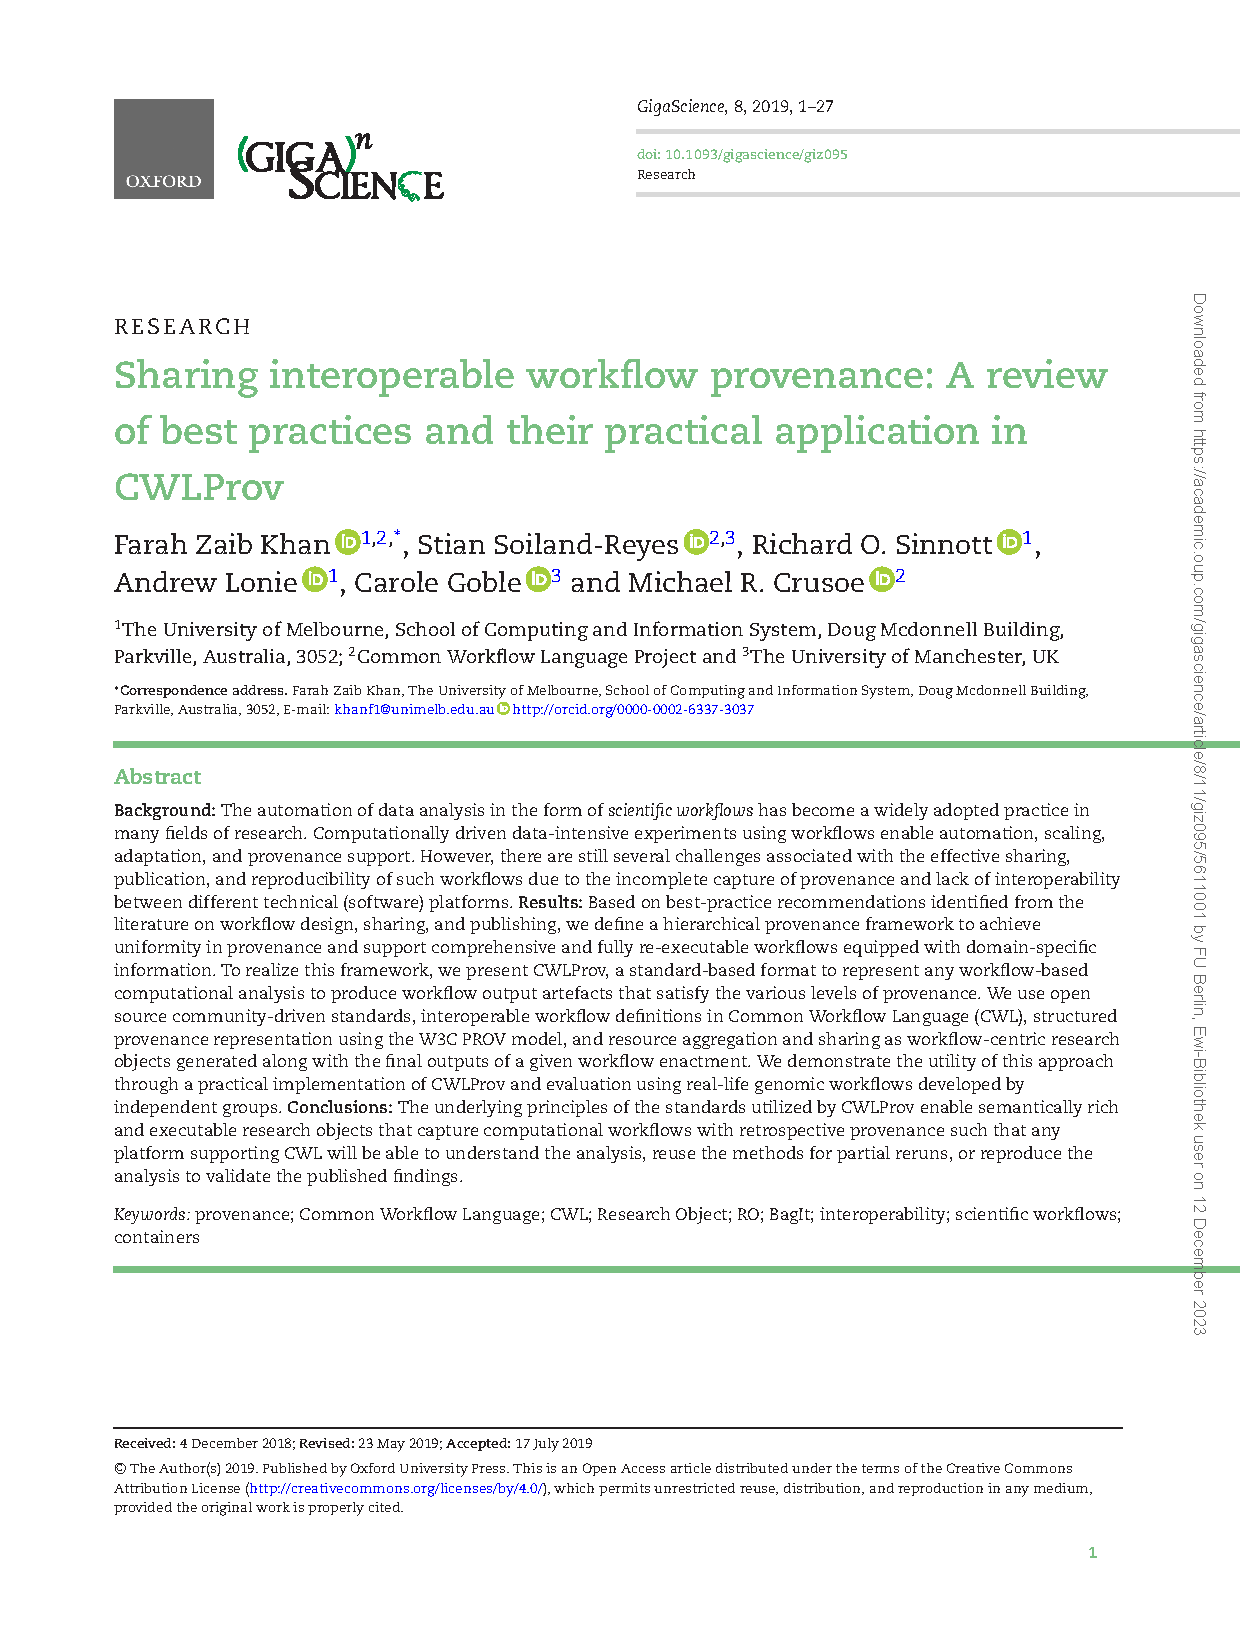
\includepdf[pages=-,addtotoc={2,section,1,Introduction,cwlprov-intro,2,section,1,Background,cwlprov-background,2,subsection,2,Provenance,cwlprov-bg-prov,2,subsection,2,Interoperability,cwlprov-bg-interop,3,subsection,2,Related Work,cwlprov-related,3,subsubsection,3,Workflow software environment capture,cwlprov-related-wfsoftenvcapture,3,subsubsection,3,Data/method {preservation,} {aggregation,} and sharing,cwlprov-related-datamethod,4,subsubsection,3,Provenance capture and standardization,cwlprov-related-provcapture,4,section,1,Levels of Provenance and Resource Sharing,cwlprov-levels-sharing,6,subsection,2,Level 0,cwlprov-level0,7,subsection,2,Level 1,cwlprov-level1,7,subsection,2,Level 2,cwlprov-level2,8,subsection,2,Level 3,cwlprov-level3,8,section,1,CWLProv 0.6.0 and Utilized Standards,cwlprov-0.6.0,9,subsection,2,Applied standards and vocabularies,cwlprov-applied-standards-vocabs,9,subsubsection,3,Common Workflow Language,cwlprov-applied-cwl,9,subsubsection,3,Research Object,cwlprov-applied-ro,10,subsubsection,3,PROV Data Model,cwlprov-applied-prov,11,subsection,2,CWLProv research object,cwlprov-cwlprovrobundle,12,subsection,2,Retrospective provenance profile,cwlprov-retroprov,12,section,1,Practical Realization of CWLProv,cwlprov-practical,14,subsection,2,Achieving recommendations with provenance levels,cwlprov-recs,15,section,1,CWLProv Evaluation with Bioinformatics Workflows,cwlprov-eval,15,subsection,2,Alignment workflow,cwlrpov-eval-alignment,16,subsection,2,Somatic variant calling workflow,cwlprov-eval-somatic,16,subsection,2,Evaluation activity,cwlprov-eval-activity,18,subsection,2,Evaluation results,cwlprov-eval-results,18,subsubsection,3,CWLProv and interoperability,cwlrpov-eval-results-interop,18,subsubsection,3,Evaluating provenance profile,cwlprov-eval-results-provprofile,19,subsubsection,3,Temporal and spatial overhead with provenance,cwlprov-eval-results-overhead,20,subsubsection,3,Output comparison across enactments,cwlprov-eval-results-output-comparison,20,section,1,Discussion and Future Directions,cwlprov-discussion,20,subsection,2,Compute and storage resources,cwlprov-discuss-resources,20,subsection,2,Provenance profile augmented with domain knowledge,cwlprov-discuss-domain,21,subsection,2,Big {-omics} data,cwlprov-discus-bigdata,21,subsection,2,Improving CWLProv efficiency with selective provenance capture,cwlprov-discuss-selective,21,subsection,2,Enforcement of best practices — an open problem,cwlprov-discuss-enforcement,22,section,1,Conclusion,cwlprov-conclusion,22,section,1,Availability of source code and requirements,cwlprov-availability-code,22,section,1,Availability of supporting data and materials,cwlprov-availability-supporting,22,section,1,Abbreviations,cwlprov-abbrevs,22,section,1,Competing interests,cwlprov-competing-interests,23,section,1,Funding,cwlprov-funding,23,section,1,Authors’ contributions,cwlprov-authors-contributions,23,section,1,Acknowledgements,cwlprov-acks,23,section,1,References,cwlprov-refs}]{giz095.pdf}  % CWLProv

\chapter{Recording provenance of workflow runs with RO-Crate}
\label{wrroc}
\bibentry{leo2023recording}

%License

Reproduced here without changes.
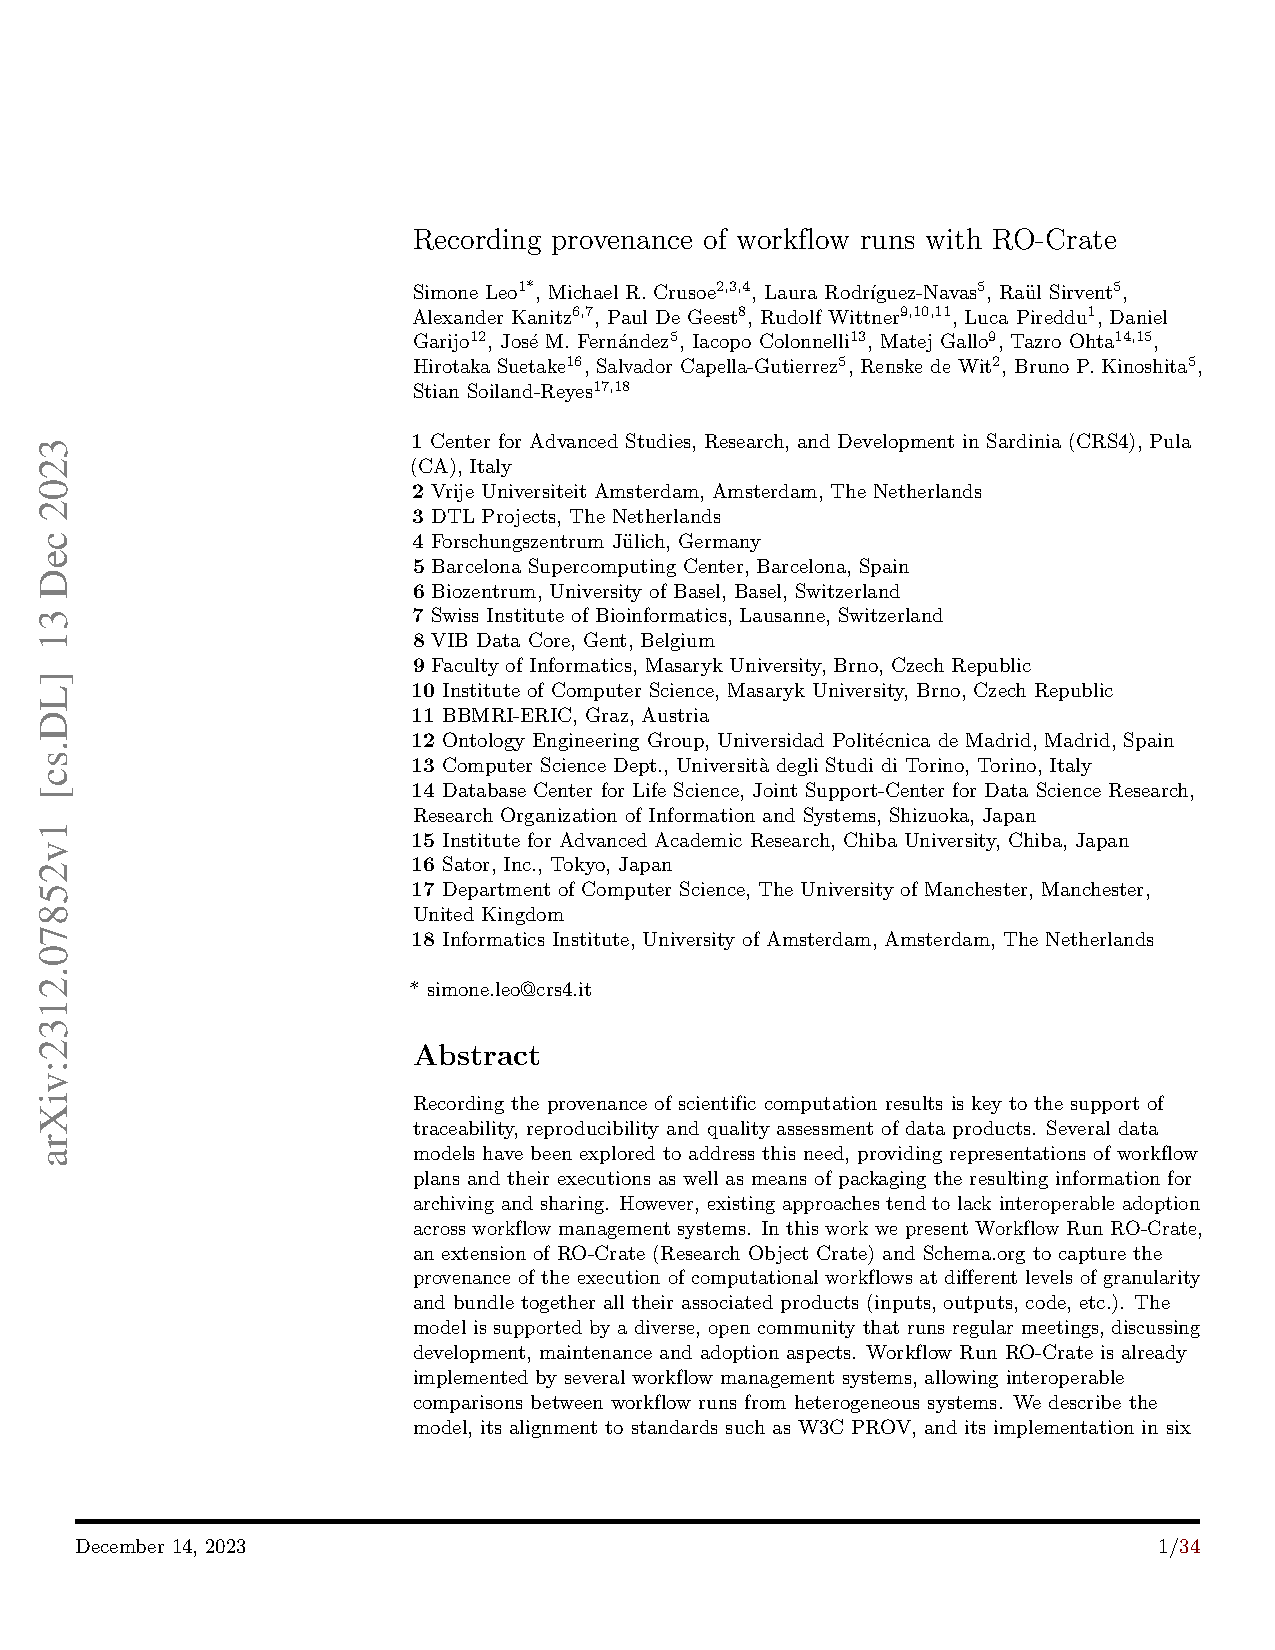
\includepdf[pages=-]{2312.07852.pdf}

\chapter{A Non-Intimidating Approach to Workflow Reproducibility in Bioinformatics: Adding Metadata to Research Objects through the Design and Evaluation of Use-Focused Extensions to CWLProv}
\label{cwlprov-analysis}
%\fullcite{}
%License
Reproduced here without changes.
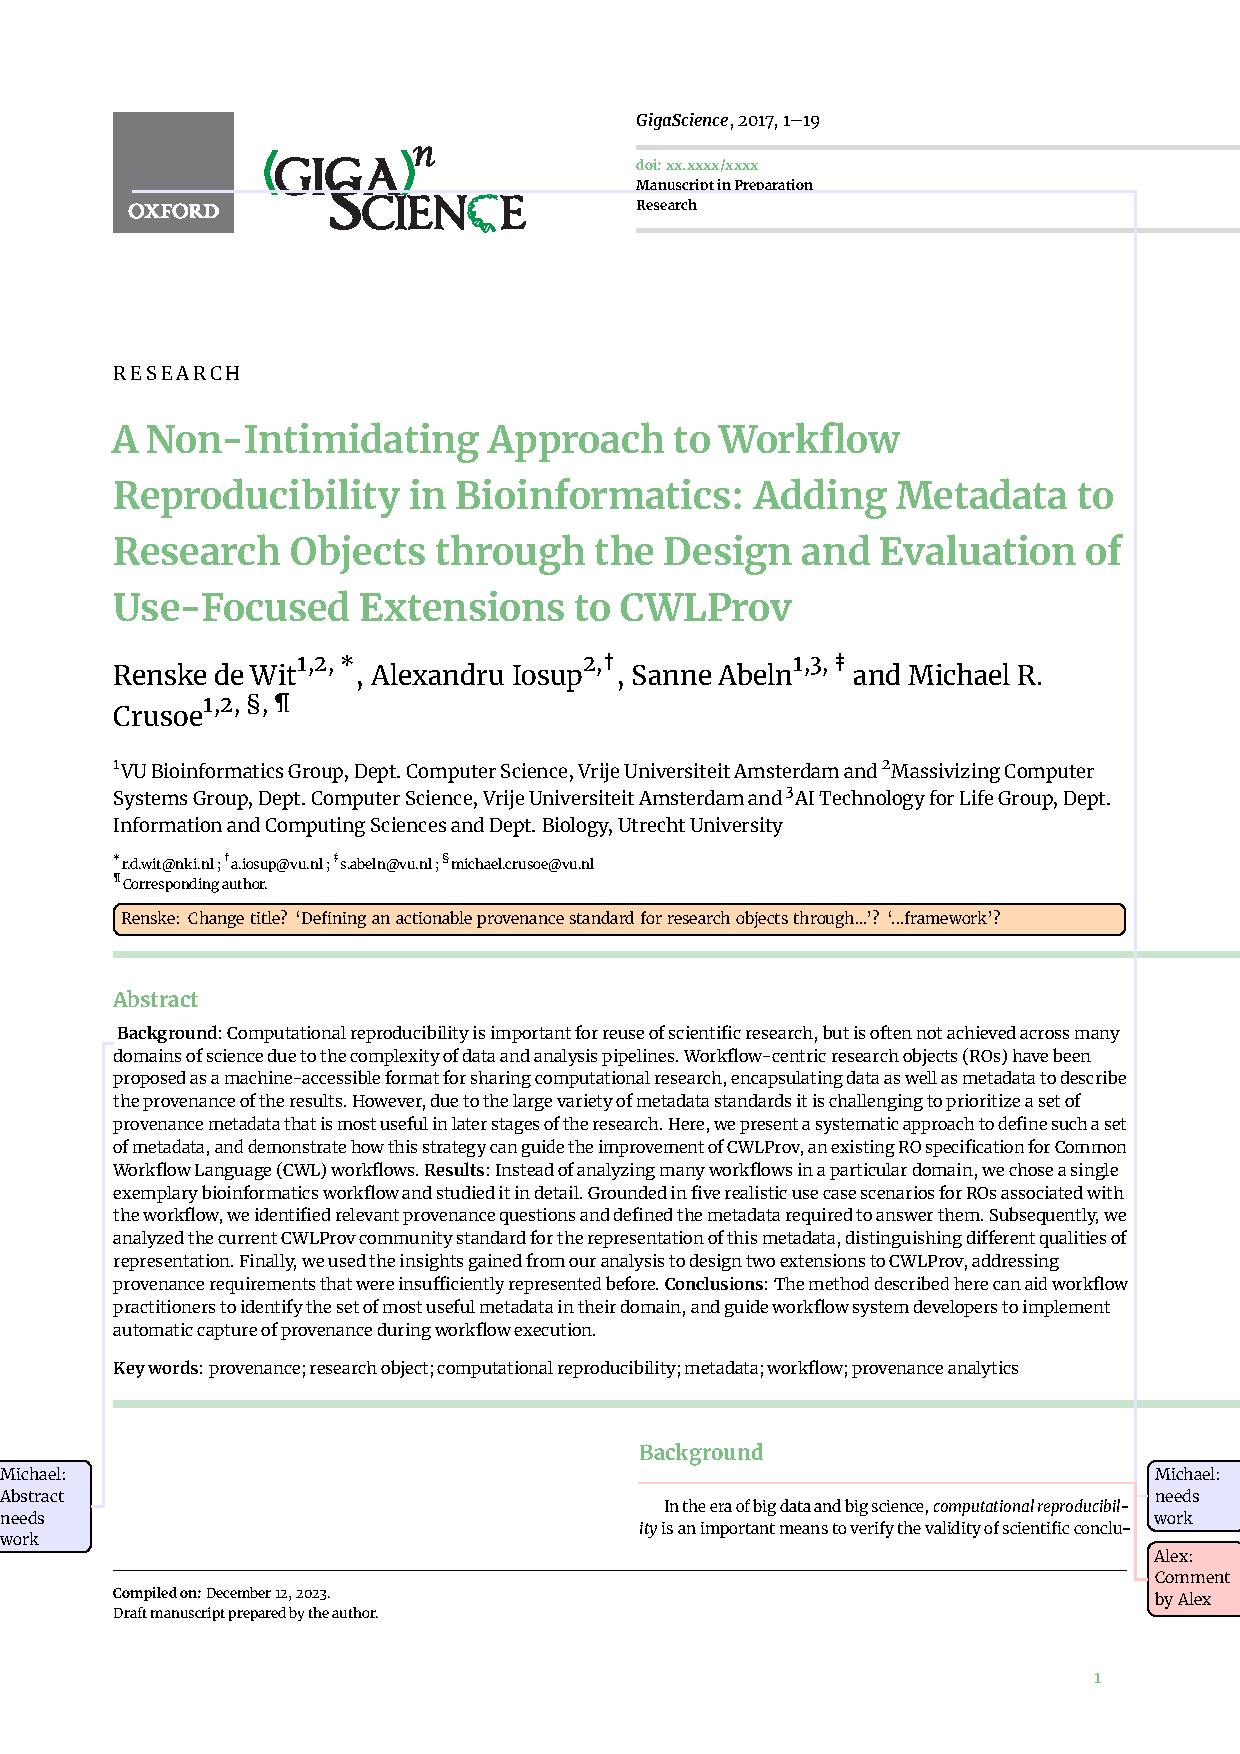
\includepdf[pages=-]{renske-cwlprov-analysis-manuscript.pdf}

\include{conclusion/conclusion}

%% Use letters for the chapter numbers of the appendices.
%\appendix

%\include{appendix-a/appendix-a}

%% Turn off thumb indices for unnumbered chapters.
\thumbfalse

\chapter*{Bibliography}
\addcontentsline{toc}{chapter}{Bibliography}
\setheader{Bibliography}

URLs in this thesis have been archived on Archive.org. Their link target in digital editions refers
to this timestamped version.

\bibliographystyle{unsrt}
% argument is your BibTeX string definitions and bibliography database(s)
\bibliography{dissertation}

%% \chapter*{Glossary}

\glsaddall
\printglossary[type=\acronymtype,title={Glossary}]
\addcontentsline{toc}{chapter}{Glossary}
\setheader{Glossary}

\include{cv/cv}
\include{publications/publications}
%\include{ipa/ipadissertations_2018}

\end{document}

